\phantomsection
\definecolor{dkgreen}{rgb}{0,0.6,0}
\definecolor{gray}{rgb}{0.5,0.5,0.5}
\definecolor{mauve}{rgb}{0.58,0,0.82}


\lstset{frame=tb,
language=R,
aboveskip=3mm,
belowskip=3mm,
showstringspaces=false,
columns=flexible,
numbers=none,
inputencoding=utf8/latin1,
keywordstyle=\color{blue},
numberstyle=\tiny\color{gray},
commentstyle=\color{dkgreen},
stringstyle=\color{mauve},
breaklines=true,
breakatwhitespace=true,
tabsize=3
}

\chapter{Criterio del Chi-quadrato}

\section{Distribuzione chi-quadrato}

Per definire la densità del chi-quadrato occorre introdurre prima la funzione $\Gamma(v)$ che è così definita:

\[\int_{0}^{\inf}x^{v-1}e^{-e}dx, \quad v>0\]

Se $v>1$ per la funzione $\Gamma(v)$ sussiste la seguente proprietà di fattorizzazione:

\[\Gamma(v) = (v-1)\Gamma(v-1) \quad (v>1)\]

La funzione gamma è una generalizzazione dei fattoriali; infatti, se $v$ è un intero positivo, usando iterativamente la formula sopracitata si ottiene

\[\Gamma(v) = (v-1)! \quad (v = 1, 2, ...)\]

Ovviamente $\Gamma(1) = 1$,

Una volta introdotta la funzione gamma è possibile presentare la funzione densità della variabile aleatoria chi-quadrato.

\noindent \textbf{Definizione:} una variabile aleatoria $X$ di probabilità

\[F_X(x) = \begin{cases}
    \frac{1}{\Gamma(n/2)}(\frac{1}{2})^{n/2-1}e^{-x/2}, & x>0.\\
    0, & x \leq 0.
    \end{cases}
    \]

dove $n$ è un intero positivo. In questo caso si parla di distribuzione chi-quadrato con $n$ gradi di libertà e si indica con $X \sim \chi^2(n)$.

Un'importante teorema afferma che la somma dei quadrati di variabili aleatorie normali standard indipendenti ha distribuzione chi-quadrato con un numero di gradi di libertà uguale al numero degli addendi, cioè:

Siano $X_1, X_2, ..., X_n$ variabili aleatorie indipendenti, con $X_i \sim N(0, 1) per i = 1, 2, ..., n$. Allora, $Y_n = X_1^2 + X_2^2 + ... + X_n^2$ ha distribuzione chi-quadrato con $n$ gradi di libertà.

Quindi, la denominazione "numero di gradi di libertà" attribuita al parametro n assume il significato di numero di addenti indipendenti presenti nella somma. 

I parametri di una variabile aleatoria chi-quadrato con $n$ gradi di libertà sono:

\[E(X) = n, \quad E(X^2)=n(n+2), \quad Var(X) = 2n\]

In R il calcolo della densità chi-quadrato viene effettuata in questo modo:

\begin{lstlisting}
    dchisq(x, df)
\end{lstlisting}

Gli argomenti passati alla funzione sono
\begin{itemize}
    \item $x$ è il valore assunto/i dalla variabile aleatoria chi-quadrato;
    \item df è il numero dei gradi di libertà.
\end{itemize}

Per calcolare la funzione di distribuzione invece utilizziamo la funzione

\begin{lstlisting}
    pchisq(x, df, lower.tail = TRUE)
\end{lstlisting}

Gli argomenti passati alla funzione sono
\begin{itemize}
    \item $x$ e il valore assunto/i dalla variabile aleatoria chi-quadrato;
    \item df è il numero dei gradi di libertà;
    \item $lower.tail$ nel caso $TRUE$ calcola $P(X\leq x)$ e nel caso $FALSE$ calcola $P(X>x)$.
\end{itemize}

Con il seguente codice si raffigura la densità di probabilità e la funzione di distribuzione di $X \sim \chi^2(n)$

\begin{lstlisting}
  par(mfrow = c(1, 2))
  curve(dchisq(x, df = 1), from = 0, to = 18, ylim = c(0, 0.3)
    , xlab = "x", ylab = "f(x)", main = "n=1,3,5,7 ")
  text(3, 0.27, "n=1")
  curve(dchisq(x, df = 3), add = TRUE, lty = 2)
  text(4, 0.20, "n=3")
  curve(dchisq(x, df = 5), add = TRUE, lty = 3) > text(6, 0.14, "n=5")
  curve(dchisq(x, df = 7), add = TRUE, lty = 4)
  text(11, 0.08, "n=7")
  curve(pchisq(x, df = 1), from = -2, to = 18, ylim = c(0, 1), xlab = "x", ylab = expression
  (P(X <= x)), main = "n=1,3,5,7 ")
  text(0, 0.9, "n=1")
  curve(pchisq(x, df = 3), add = TRUE, lty = 2)
  arrows(4, 0.7, 12, 0.8, code = 1, length = 0.10)
  text(14, 0.8, "n=3")
  curve(pchisq(x, df = 5), add = TRUE, lty = 3)
  arrows(5.5, 0.6, 13, 0.7, code = 1, length = 0.10)
  text(15, 0.7, "n=5")
  curve(pchisq(x, df = 7), add = TRUE, lty = 4)
  text(8, 0.4, "n=7")
\end{lstlisting}

ottenendo il seguente grafico

\begin{figure}[!htb]
    \centering
    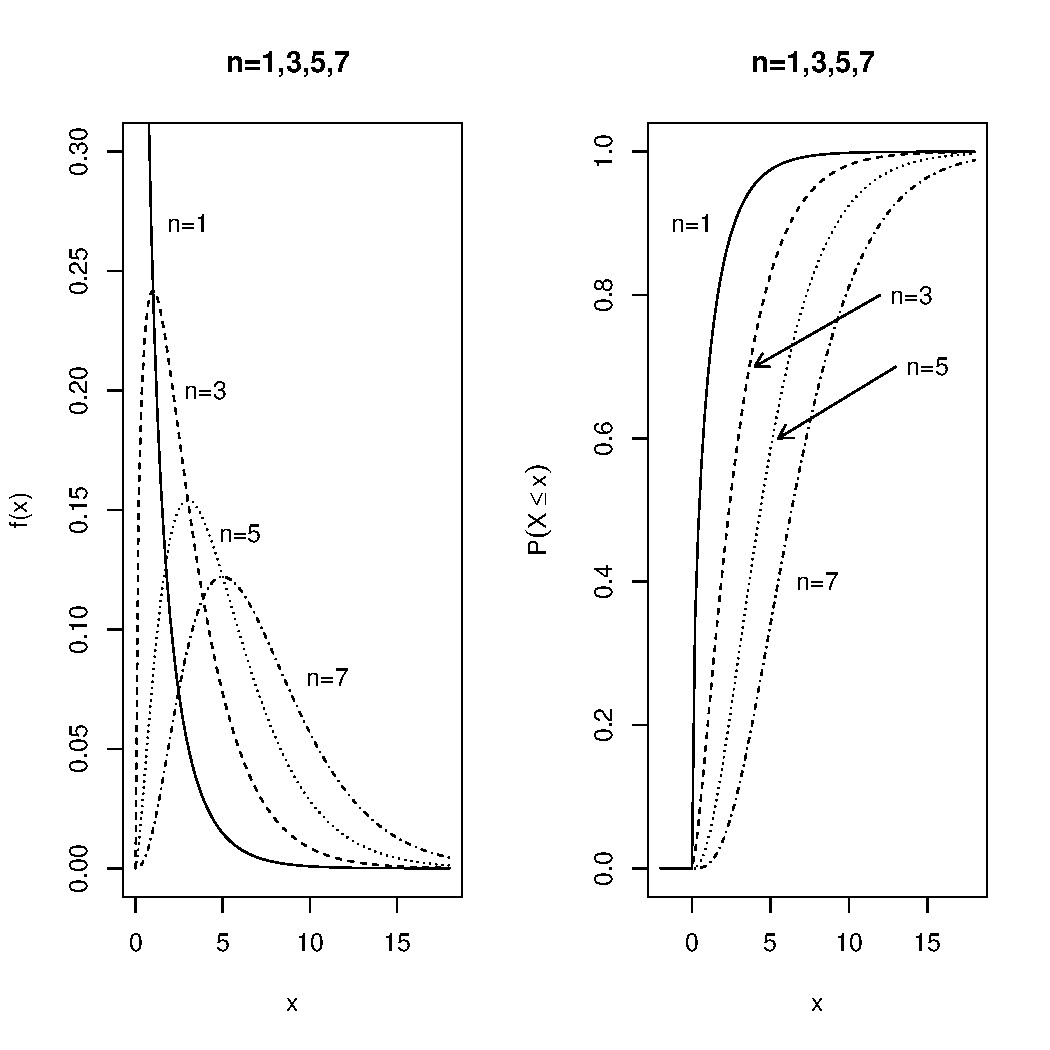
\includegraphics[height=16cm]{capitoli/images/4_chiquadrato/densProbChi.pdf}
    \caption{Densità di probabilità e funzione di distribuzione}
\end{figure}

In molti problemi reali, si desidera verificare se il campione osservato può essere stato estratto da una popolazione descritta da una variabile aleatoria $X$ con funzione di distribuzione $F_X(x)$. A questo scopo, si utilizza il criterio di verifica delle ipotesi del chi-quadrato, detto anche test del chi-quadrato o test del buon adattamento.

\section{Criterio del chi-quadrato bilaterale}

Con il criterio del  chi-quadrato si desidera verificare l'ipotesi che una certa popolazione, descritta da una variabile aleatoria $X$, sia caratterizzata da una funzione di distribuzione $F_X(x)$ con $k$ parametri non noti da stimare. Denotando con $H_0$ l'ipotesi soggetta a verifica (ipotesi nulla) e con $H_1$ l'ipotesi alternativa, il test chi-quadrato di misura $\alpha$ mira a verificare l'ipotesi nulla.

$H_0:X$ ha una funzione di distribuzione $F_X(x)$ (avendo stimato k parametri non noti in base al campione) 

in alternativa all'ipotesi

$H_1:X$ non ha una funzione di distribuzione $F_X(x)$ dove $\alpha$ è la probabilità massima di rifiutare l'ipotesi nulla quando essa è vera.

Anche in questo caso si determina un test $\phi$ di misura $\alpha$ che permetta di determinare una regione di accettazione e di rifiuto dell'ipotesi nulla. 

Si suddivida l'insieme dei valori che la variabile aleatoria $X$ può assumere in $r$ sottoinsiemi $I_1, I_2, ..., I_r$ in modo che risulti essere uguale a $p_i$ la probabilità che, secondo la distribuzione ipotizzata, la variabile aleatoria assuma un valore appartenente a $I_i$, ossia

\[p_i = P(X \in I_i) \quad (i=1,2,...,r\].

Lo step successivo, preso un campione $x_1, x_2, ..., x_n$ è di calcolare le frequenze assolute $n_2, ..., n_r$ con cui gli $n$ elementi si distribuiscono nei rispettivi insiemi $I_1, I_2, ..., I_r$. Il numero medio di elementi che cadono nell'intervallo $I_i$ è $np_i$. Si calcola poi la quantità

\[x^2 = \sum_{i=1}^r(\frac{n_i - np_i}{\sqrt{np_i}})^2\]

Il criterio chi-quadrato si basa sulla statistica

\[Q = \sum_{i=1}^r(\frac{N_i - np_i}{\sqrt{np_i}})^2\]

dove $N_i$ è la variabile aleatoria che descrive il numero degli elementi del campione casuale $X_1, X_2, ..., X_n$ (costituito da $n$ variabili  aleatorie osservabili, indipendenti e identicamente distribuite con la stessa legge di probabilità $F_X(x)$ della popolazione) che cadono nell'intervallo $I_i(i=1,2,...,r)$.

Se la variabile aleatoria $X$ ha una funzione di distribuzione $F_X(x)$ con $k$ parametri non noti, si può dimostrare che per $n$ sufficientemente grande la funzione di distribuzione della statistica $Q$ è approssimabile con la funzione di distribuzione chi-quadrato con $r-k-1$ gradi di libertà.

Per garantire che ogni classe contenga almeno 5 elementi, si ritiene valida l'approssimazione se risulta 

\[min(np_1, np_2, ..., np_r) \geq 5\]

Si giunge così alla definizione del test chi-quadrato bilaterale. Per un campione sufficientemente numeroso di ampiezza $n$, il test chi-quadrato bilaterale di misura $\alpha$ è il seguente:

\begin{itemize}
    \item si rifiuti l'ipotesi $H_0 se \chi^2 < \chi_{1-\alpha/2,r-k-1}^2$ oppure $\chi^2 > \chi_{\alpha/2, r-k-1}^2$;
    \item si accetti l'ipotesi $\chi_{1-\alpha/2,r-k-1}^2 < \chi^2 < \chi_{\alpha/2, r-k-1}^2$
\end{itemize}

dove $\chi_{1-\alpha/2,r-k-1}^2$ e $\chi_{\alpha/2,r-k-1}^2$ sono soluzioni dele equazioni:

\[P(Q<\chi_{1-\alpha/2,r-k-1}^2) = \frac{\alpha}{2}, \quad P(Q<\chi_{\alpha/2,r-k-1}^2) = 1-\frac{\alpha}{2}\]

\noindent \textbf{Esempio}

\begin{lstlisting}
[1] 2.5889415 2.4274552 2.2879886 2.5257274 1.3608815 1.8330865 2.2110392
[8] 2.9302882 2.1603784 2.8153400 1.2379034 1.3232095 1.5533711 1.1738130
[15] 1.1798547 2.0803117 1.4592185 1.5569350 1.4902865 2.0316545 2.4187870
[22] 2.5316882 3.0833015 1.8875859 1.5517724 3.0869650 2.1161441 2.2039643
[29] 1.0669755 2.0200946 2.5388058 2.3822110 2.1206882 1.6142661 2.3803540
[36] 2.4263595 2.8091048 1.5316683 1.6807372 2.7404029 1.5801006 1.8411243
[43] 1.9379254 2.2090764 1.8581314 2.2168108 2.4149075 1.8682822 2.4080365
[50] 2.5663934 1.7010245 1.8328371 1.9498204 1.5384879 1.6274098 2.4448616
[57] 1.6637135 3.1919928 1.2788193 1.6247899 1.8259281 2.1353790 2.0575756
[64] 2.2415920 2.6733718 1.0493558 1.7638138 2.3932882 1.8392844 2.2664697
[71] 1.8736283 1.3277308 1.8608656 2.1320640 1.3944918 1.5087226 2.2219716
[78] 0.9680605 2.1960015 1.8015670

  n <- length(ds)
  n
  [1] 80

  m <- mean(ds)
  m
  [1] 1.996316

  d <- sd(ds)
  d
  [1] 0.51082
\end{lstlisting}

Applicando il test chi-quadrato di misura $\alpha = 0.05$ si desidera verificare se la popolazione da cui proviene il campione può essere descritta da una variabile aleatoria $X$ di densità normale

\[f_X(x) = \frac{1}{\delta \sqrt{2\pi}}exp{-\frac{(x-\mu)^2}{2\delta^2}}, \quad x \in \mathbb{R} \quad (\mu \in \mathbb{R}, \delta>0)\]

Supponiamo di suddividere l'insieme dei valori che tale variabile aleatoria normale $X$ può assumere in $r=4$ sottoinsiemi $I_1, I_2, ..., I_4$ in modo che risulti essere uguale a $p_i=0.25$ la probabilità che $X$ assuma un valore appartenente a $I_i(i=1,2,...,4)$. La condizione è verificata essendo $npi = 80*0.25 = 20\geq4$. Ricordando che uno stimatore di $\mu$ è la media campionaria e uno stimatore di $\delta^2$ è la varianza campionaria, utilizzando i quantili della distribuzione normale possiamo determinare i sottoinsiemi $I_1, I_2, ..., I_4$

\begin{lstlisting}
  quantili <- numeric(3)
  for (i in 1:3)
    quantili[i] <- qnorm(0.25 * i, mean = m, sd = d)
  quantili

  [1] 1.651773 1.996316 2.340859
\end{lstlisting}

Gli intervalli $I_1, I_2,..., I_4$ sono:

\[I_1 = (-\inf, 1.65), \quad I_2=[1.65, 2.00)\]
\[I_3 = [2.00,2.34), \quad I_4 = [2.34,+\inf)\]

Occorre ora determinare il numero di elementi del campione che cadono negli intervalli $I_1, I_2, ..., I_4$:

\begin{lstlisting}
  r <- 4
  nint <- numeric(r)
  nint[1] <- length(which(ds < quantili[1]))
  nint[2] <- length(which((ds >= quantili[1]) & (ds < quantili[2])))
  nint[3] <- length(which((ds >= quantili[2]) & (ds < quantili[3])))
  nint[4] <- length(which((ds >= quantili[3])))
  nint

  [1] 23 17 18 22
\end{lstlisting}

Con il seguente codice si raffigurano le classi che suddividono il campione:

\begin{lstlisting}
  curve(dnorm(x, mean = m, sd = d), from = -1.25, to = 5.25,
        axes = FALSE, ylim = c(0, 0.8), xlab = "", ylab = "",
        main = "Densita normale mu = 1.99 sigma = 0.51")
  axis(side = 1, labels = FALSE)
  axis(side = 2, labels = TRUE)
  lines(x = quantili, y = dnorm(quantili, mean = m, sd = d), type = "h", lty = 2, xlab = "")
  axis(1, at = quantili, round(quantili, digits = 2), las = 2, cex.axis = 0.8)
\end{lstlisting}

\begin{figure}[!htbp]
    \centering
    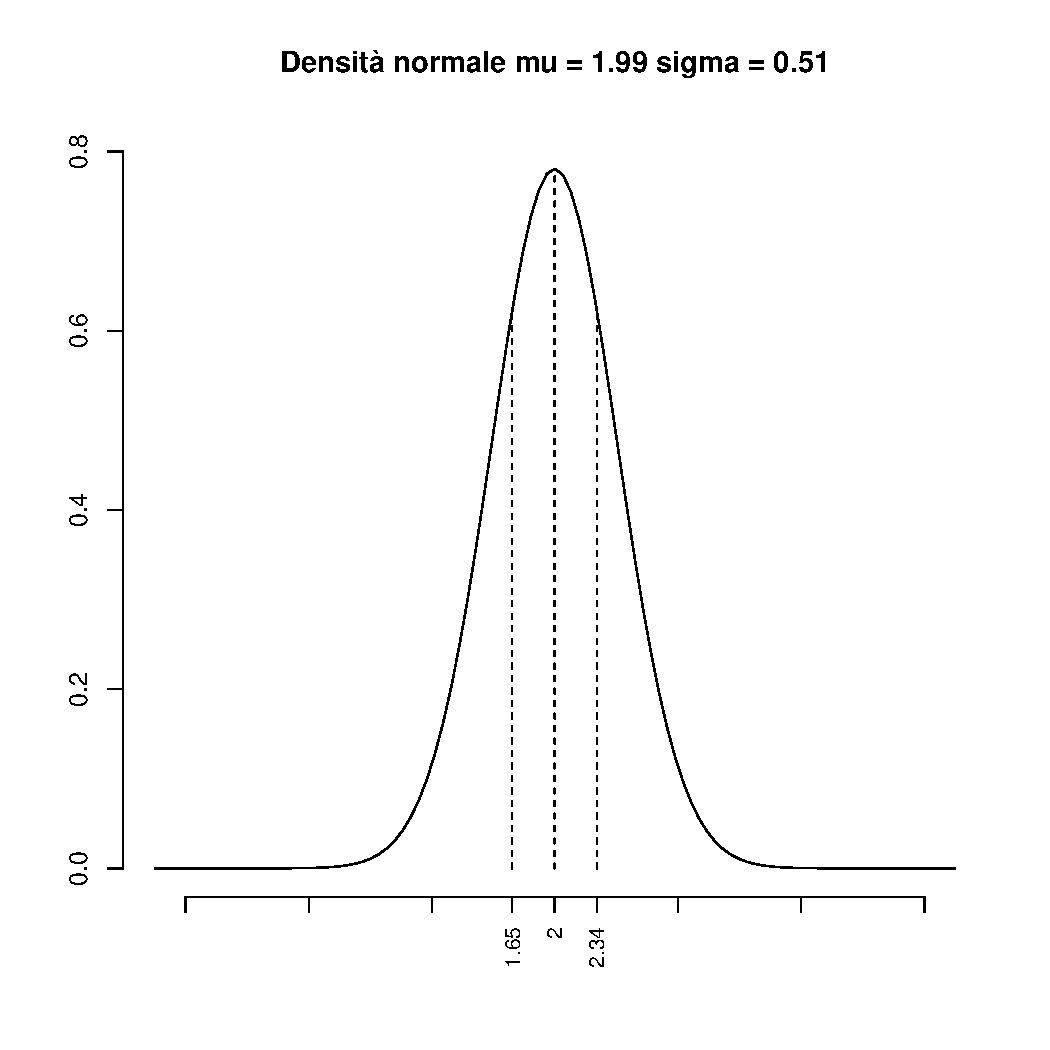
\includegraphics[height=16cm]{capitoli/images/4_chiquadrato/densNorm.pdf}
    \caption{Rappresentazione grafica dei 4 intervalli}
\end{figure}

Calcoliamo ora $\chi^2$

\begin{lstlisting}
  chi2 <- sum(((nint - n * 0.25) / sqrt(n * 0.25))^2)
  chi2
  [1] 1.3
\end{lstlisting}

La distribuzione normale ha due parametri non noti $(\mu, \delta^2)$ e quindi $k=2$. Pertanto, la funzione di distribuzione della statistica $Q$ è approssimabile con la funzione di distribuzione chi-quadrato con $r-k-1=2$ gradi di libertà. La funzione $qchisq$ permette di calcolare i quantili di una funzione di distribuzione chi-quadrato.

Occorre quindi calcolare $\chi_{\alpha/2,2}^2$ e $\chi_{1-\alpha/2,2}^2$ con $\alpha = 0.05$

\begin{lstlisting}
  k <- 2
  alpha <- 0.05
  qchisq(alpha / 2, df = r - k - 1)
  [1] 0.0009820691
  qchisq(1 - alpha / 2, df = r - k - 1)
  [1] 5.023886
\end{lstlisting}

da cui segue che $\chi_{\alpha/2,2}^2 = 0.000982$ e $\chi_{1-\alpha/2,2}^2 = 5.0239$. Essendo $0.000982 < 1.3 < 5.0239$ l'ipotesi $H_0$ di popolazione normale deve essere accettata. Di seguito la rappresentazione grafica della regione di accettazione.

\begin{lstlisting}
  curve(dchisq(x, df = 2), from = 0, to = 10, ylim = c(0, 0.6), xlab = "", axes = FALSE, ylab = "",
        main = "Densita di Chi-Quadrato con 2 gradi di liberta")
  axis(side = 1, labels = FALSE)
  axis(side = 2, labels = FALSE)
  axis(1, at = qchisq(alpha / 2, df = r - k - 1), "chi^2 alpha/2,2")
  axis(1, at = qchisq(1 - alpha / 2, df = r - k - 1), "chi^2 1-alpha/2,2")
  lines(x = c(0.0009820691, 5.023886), y = dchisq(c(0.0009820691, 5.023886), df = 2), type = "h", lty
    = 2, xlab = "")
  text(2, 0.04, expression("Reg. accettazione"))
  lines(x = 1.3, y = dchisq(1.3, df = 2), type = "h", lty = 2, xlab = "")
  axis(1, at = 1.3, "1.3")
\end{lstlisting}

\begin{figure}[!htbp]
    \centering
    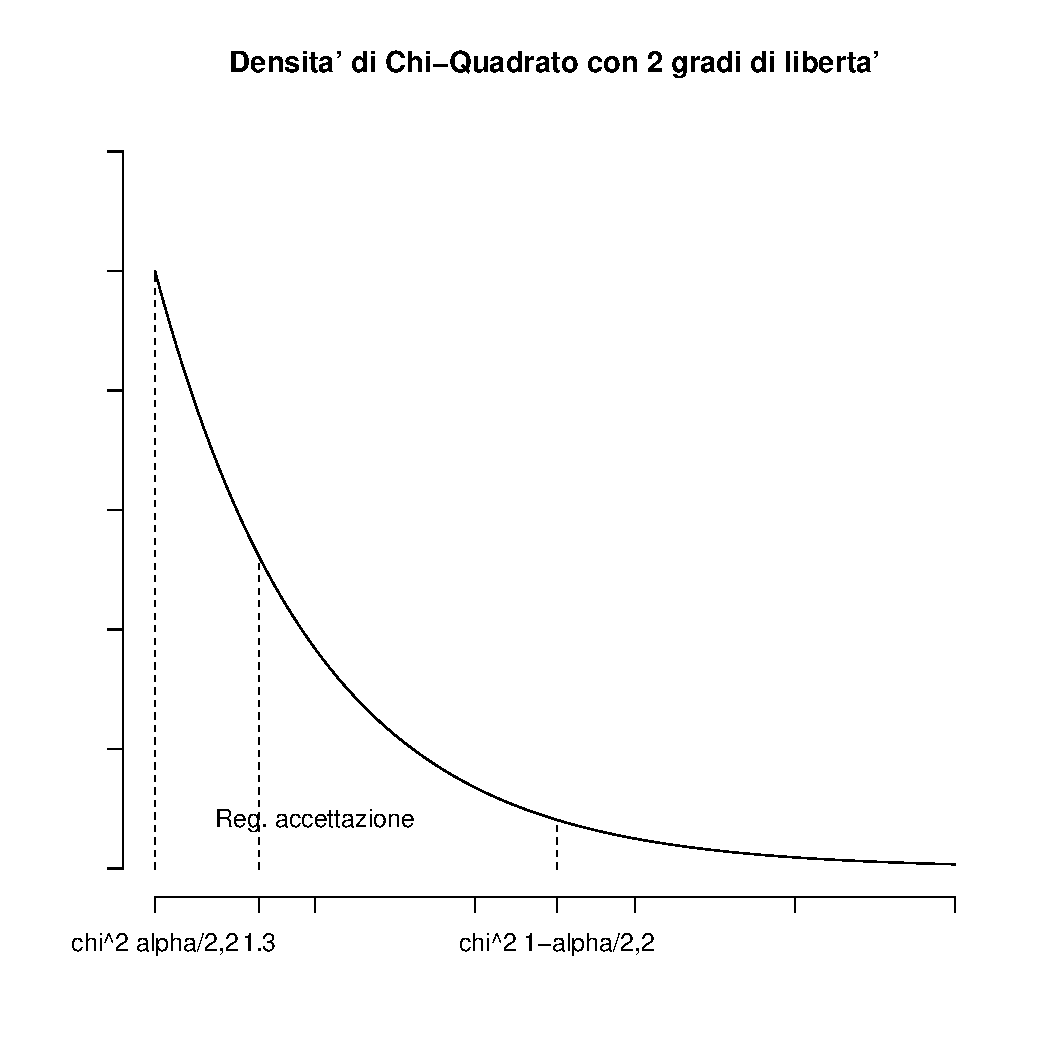
\includegraphics[height=16cm]{capitoli/images/4_chiquadrato/densChiFinal.pdf}
    \caption{ Regione di accettazione con grado di confidenza 0.05
}
\end{figure}

Essendo $0.000982 < \chi^2 < 5.0239$, l'ipotesi $H_0$ di popolazione normale può essere accettata.

%################################################

\newpage